\documentclass{ctexart}
\usepackage{PhysicalChemistryNote}

\begin{document}\pagestyle{plain}
\noindent\tbf{\LARGE 6A 电解质溶液}\vspace{15pt}\\
\indent 电解质溶液,例如食盐水,具有普通溶液所不具有的导电性,%
这是因为溶液中的\ce{Na^+}和\ce{Cl^-}在电场的作用下能发生定向移动,起到传递电荷的作用.%
除此之外,带异种电荷的离子之间还存在吸引力,带同种电荷的离子之间还存在排斥力.%
以上种种原因,都使得电解质溶液与一般的溶液性质并不完全相似.因此,%
我们将在本节简单的讨论其性质.\vspace{12pt}\\
\Section{6A.1 电解质溶液的电导}
\Part{电导,电导率和摩尔电导率}
\indent 物质的导电能力,通常用电阻$R$来表示.而对于电解质溶液,我们更希望直观地判断其导电能力,%
这一物理量越大,电解质溶液的导电能力就越强.因此,可以定义\tbf{电导}来衡量其导电能力.
\begin{definition}[6A.1.1 电导]
    \tbf{电导}$G$定义为电阻$R$的倒数,即$G=\dfrac1R$.
\end{definition}
导体的电阻与其长度$l$成正比,与其横截面积$S$成反比,比例系数为电阻率$\rho$,它与导体的材料有关.于是
\[R=\rho\dfrac{l}{S}\]
因此,物体的电导
\[G=\dfrac{1}{\rho}\dfrac{S}{l}\]
同样地,可以定义\tbf{电导率}以衡量材料的导电能力.
\begin{definition}[6A.1.2 电导率]
    \tbf{电导率}$\kappa$定义为电阻率$\rho$的倒数,即$\kappa=\dfrac{1}{\rho}$.
\end{definition}
对于不同浓度的溶液,其中离子的数目不同,因而导电性也是不同的.%
因此,可以定义\tbf{摩尔电导率}.
\begin{definition}[6A.1.3 摩尔电导率]
    \tbf{摩尔电导率}$\varLambda_\m$定义为溶液电阻率与摩尔浓度的之比,即$\varLambda_\m=\dfrac{\kappa}{c}$.\\
    摩尔电导率的操作定义\footnotemark 为在两个相距$1\text{ m}$的平行电极板之间充入含有$1\mol$电解质的一定浓度的溶液时具有的电导.
\end{definition}\footnotetext{操作定义,是根据可观察,可测量,可操作的特征来界定变量含义的方法.}
在讨论摩尔电导率时,需要指定电解质的基本单元.例如$\varLambda_\m(\ce{NaCl})$和$\displaystyle\varLambda_\m\left(\ce{1/2NaCl}\right)$%
在操作定义中分别指\ce{NaCl}为$1\mol$和\ce{Na^+}与\ce{Cl^-}的总量为$1\mol$.对于同一浓度的\ce{NaCl}溶液,有
\[\varLambda_\m(\ce{NaCl})=2\varLambda_\m\left(\ce{1/2NaCl}\right)\]
\Part{电导率,摩尔电导率与浓度的关系}
\indent 我们先讨论浓度与电导率的关系.几种典型的电解质溶液的电导率与浓度的关系如下图所示.
\begin{tightcenter}
    \documentclass{standalone}
\usepackage{PhysicalChemistryNote}
\begin{document}
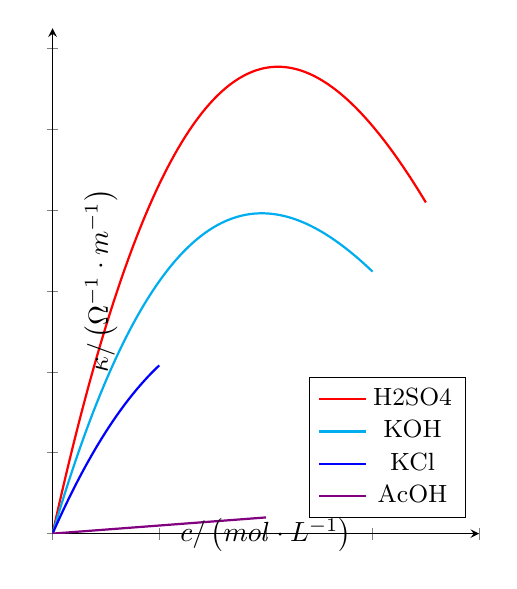
\begin{tikzpicture}
    \begin{axis}[
        width = 7cm,
        height = 8cm,
        legend pos = south east,
        xlabel = {$c/\left(\text{mol}\cdot\text{L}^{-1}\right)$},
        ylabel = {$\kappa/\left(\Omega^{-1}\cdot\text{m}^{-1}\right)$},
        axis lines = left,
        x label style={at={(axis description cs:0.5,0.05)},anchor=north},
        y label style={at={(axis description cs:0.175,0.5)},rotate=0,anchor=south},
        ymax = 1.25,
        ymin = 0,
        xmax = 0.8,
        ymin = 0,
        samples = 400,
        xticklabels={},
        yticklabels={}
    ]
    \addplot [thick, red, domain=0:0.7] {3*x*(x-1)*(x-2)};
    \addlegendentry{\small{\ce{H2SO4}}}
    \addplot [thick, cyan, domain=0:0.6] {3*x*(x-1)*(x-1.5)};
    \addlegendentry{\small{\ce{KOH}}}
    \addplot [thick, blue, domain=0:0.2] {2*x*(x-1)*(x-1.5)};
    \addlegendentry{\small{\ce{KCl}}}
    \addplot [thick, violet, domain=0:0.4] {0.1*x};
    \addlegendentry{\small{\ce{AcOH}}}
    \end{axis}
\end{tikzpicture}
\end{document}
\end{tightcenter}
可以看出,在一定浓度范围内,强电解质的电导率$\kappa$随浓度的上升而上升,%
这是由于溶液中离子的浓度上升使得导电的粒子数增多;超过一定浓度范围后,$\kappa$随浓度增大而减小,%
这是由于离子变得密集,正负离子间的吸引力增大,限制了离子的导电能力所致.\\
\indent 对于弱电解质而言,$\kappa$随浓度变化不显著.浓度增大,虽然单位体积溶液的电解质分子数增多,%
但电离度却随之减小,因此离子的浓度变化不大.\\
\indent 与电导率所不同,电解质的摩尔电导率$\varLambda_\m$却总是随着浓度的增加而减小.%
几种典型的电解质溶液的电导率与浓度的关系如下图所示(注意这里的横坐标为$\sqrt{c}$).
\begin{tightcenter}
    \documentclass{standalone}
\usepackage{PhysicalChemistryNote}
\begin{document}
\begin{tikzpicture}
    \begin{axis}[
        width = 8cm,
        height = 8cm,
        legend style={at={(1.05,0.5)},anchor=west},
        xlabel = {$\sqrt{c}$},
        ylabel = {$\varLambda_\m$},
        axis lines = left,
        x label style={at={(axis description cs:0.5,0.05)},anchor=north},
        y label style={at={(axis description cs:0.175,0.5)},rotate=0,anchor=south},
        ymax = 0.5,
        ymin = 0,
        xmax = 0.6,
        ymin = 0,
        samples = 400,
        xticklabels={},
        yticklabels={}
    ]
    \addplot [thick, red, domain=0:0.6] {e^(-x-3)-e^(-3)+0.45};
    \addlegendentry{\small{\ce{HCl}}}
    \addplot [thick, cyan, domain=0:0.6] {e^(-x-1)-e^(-1)+0.45};
    \addlegendentry{\small{\ce{H2SO4}}}
    \addplot [thick, blue, domain=0:0.6] {e^(-x-2)-e^(-2)+0.2};
    \addlegendentry{\small{\ce{Na2SO4}}}
    \addplot [thick, violet, domain=0:0.6] {0.4/(1+100*x)};
    \addlegendentry{\small{\ce{AcOH}}}
    \addplot [domain=0:0.6,dashed] {-e^(-3)*x+0.45};
    \addplot [domain=0:0.6,dashed] {-e^(-1)*x+0.45};
    \addplot [domain=0:0.6,dashed] {-e^(-2)*x+0.2};
    \end{axis}
\end{tikzpicture}
\end{document}
\end{tightcenter}

\indent 对于强电解质,浓度上升时两电极间的电解质数量仍保持$1\mol$,参加导电的离子数目没有变化,%
而浓度上升,离子间引力变大,离子迁移速度略有减小,于是$\varLambda_\m$随着$\sqrt{c}$的增加而缓慢减小.\\
\indent 对弱电解质,浓度上升时虽然电极间的电解质数量不变,但电离度大大减小,
导致参加导电的离子数目大大减少,于是$\varLambda_\m$随着$\sqrt{c}$的增加而迅速减小.\\
\indent 另外,可以发现当浓度$c$趋近于$0$时,各种物质的摩尔电导率都趋近于一定值,这一值记为\tbf{极限摩尔电导率}.
\begin{definition}[6A.1.4 极限摩尔电导率]
    电解质溶液在浓度趋于$0$时的摩尔电导率也趋于某一定值(即溶液无限稀释时的摩尔电导率),%
    这一定值记为该电解质溶液的\tbf{极限摩尔电导率},记为$\varLambda_\m^\infty$.
\end{definition}
Kohlrausch发现对于强电解质而言,在浓度较低时$\varLambda_\m$与$\sqrt{c}$呈现线性关系,即
\[\varLambda_\m=\varLambda_\m^\infty\left(1+\beta\sqrt{c}\right)\]
我们在上图中也标出了相应的虚线以直观地表现这一关系.因此,取浓度较低时的几组$\varLambda_\m$-$\sqrt{c}$数据,%
线性回归得到直线后外推至$c=0$即可得到对应的$\varLambda_\m^\infty$.\\
\indent 然而,对于弱电解质,稀释时伴随着电解质的电离.即使在很稀的时候,$\varLambda_\m$仍然与$\sqrt{c}$没有明显的线性关系,%
上述外推法求$\varLambda_\m^\infty$有很大的误差.Kohlrausch提出的离子独立移动定律解决了这一点.%
他发现以下关系
\[\varLambda_\m^\infty(\ce{HCl})-\varLambda_\m^\infty(\ce{HNO3})
=\varLambda_\m^\infty(\ce{KCl})-\varLambda_\m^\infty(\ce{KNO3})
=\varLambda_\m^\infty(\ce{LiCl})-\varLambda_\m^\infty(\ce{LiNO3})=\cdots\]
即无限稀释后\ce{Cl^-}和\ce{NO3^-}对$\varLambda_\m^\infty$的贡献之差相同,不会因为正离子的改变而改变.%
对于负离子,这一关系仍然成立.因此,Kohlrausch假定各种离子在无限稀释具有恒定的$\varLambda_\m^\infty$,%
电解质的$\varLambda_\m^\infty$就是组成它的各种离子的$\varLambda_\m^\infty$之和.
\begin{theorem}[6A.1.5 离子独立移动定律]
    电解质的$\varLambda_\m^\infty$就是组成它的各种离子的$\varLambda_\m^\infty$之和.对于组成为\ce{M_{$\nu_+$}X_{$\nu_-$}}的电解质,其极限摩尔电导率
    \[\varLambda_\m^\infty=\nu_+\varLambda_{\m,+}^\infty+\nu_-\varLambda_{\m,-}^\infty\]
    其中$\varLambda_{\m,+}^\infty$和$\varLambda_{\m,-}^\infty$分别为两种离子各自的极限摩尔电导率.
\end{theorem}
这样,对于弱电解质就可以间接地求出其$\varLambda_\m^\infty$.以\ce{AcOH}为例,有
\[\begin{aligned}
    \varLambda_\m^\infty(\ce{AcOH})
    &= \varLambda_\m^\infty(\ce{H^+})+\varLambda_\m^\infty(\ce{AcO^-}) \\
    &= \left(\varLambda_\m^\infty(\ce{H^+})+\varLambda_\m^\infty(\ce{Cl^-})\right)
        +\left(\varLambda_\m^\infty(\ce{Na^+})+\varLambda_\m^\infty(\ce{AcO^-})\right)
        -\left(\varLambda_\m^\infty(\ce{Na^+})+\varLambda_\m^\infty(\ce{Cl^-})\right) \\
    &= \varLambda_\m^\infty(\ce{HCl})+\varLambda_\m^\infty(\ce{AcONa})-\varLambda_\m^\infty(\ce{NaCl})
\end{aligned}\]
而\ce{HCl},\ce{AcONa}和\ce{NaCl}都是强电解质,因此后面的三个数据都是容易得到的.\vspace{4pt}\\
\Part{电导率测定的应用}
\indent 电导率测定可以求算弱电解质的解离度和解离常数.
\begin{derivation}
    在弱电解质溶液中,只有已经解离成离子的部分才能承担导电的任务.电导率与离子浓度成正比,即$\kappa=kc_{\text{ion}}$%
    (我们在\tbf{6A.2}中将会知道这可以由电迁移率推出).%
    设弱电解质在某一条件下的解离度为$\alpha$,无限稀释时的解离度$\alpha^\infty=1$,则有
    \[\dfrac{\varLambda_\m}{\varLambda_\m^\infty}
    =\dfrac{\dfrac{\kappa}{c}}{\dfrac{\kappa^\infty}{c^\infty}}
    =\dfrac{k\dfrac{c_{\text{ion}}}{c}}{k\dfrac{c_{\text{ion}}^\infty}{c^\infty}}
    =\dfrac{\alpha}{\alpha^\infty}=\alpha\]
    即摩尔电导率$\varLambda_\m$与极限摩尔电导率$\varLambda_\m$的比值为$\alpha$.\\
    我们考虑$1:1$型电解质\ce{MX},其电离平衡
    \begin{tightcenter}
        \ce{MX <=> M^+ + X^-}
    \end{tightcenter}
    设\ce{MX}的分析浓度为$c$,则有
    \[K^\ominus=\dfrac{c(\ce{M^+})c(\ce{X^-})}{c(\ce{MX})c^\ominus}
    =\dfrac{c\alpha^2}{c^\ominus(1-\alpha)}
    =\dfrac{\varLambda_\m^2}{\varLambda_\m^\infty\left(\varLambda_\m^\infty-\varLambda_\m\right)}\cdot\dfrac{c}{c^\ominus}\]
    上式亦可以改写为便于线性回归的形式,即
    \[\dfrac{1}{\varLambda_\m}=\dfrac{1}{\varLambda_\m^\infty}+\dfrac{1}{c^\ominus K^\ominus\left(\varLambda_\m^\infty\right)^2}\cdot c\varLambda_\m\]
    以$\dfrac{1}{\varLambda_\m}$对$c\varLambda_\m$线性回归即可得$K^\ominus$.在求算$K^\ominus$时,%
    尽量代入查阅手册的$\varLambda_\m^\infty$(这是由前面的离子独立移动定律得到的),因为线性回归得到的$\varLambda_\m^\infty$并不那么准确.
\end{derivation}
上述结论就是Ostwald稀释定律.
\begin{theorem}[6A.1.6 Ostwald稀释定律]
    ($1:1$型的)弱电解质的解离平衡常数$K^\ominus$与解离度$\alpha$满足
    \[K^\ominus=\dfrac{\alpha^2}{1-\alpha}\cdot\dfrac{c}{c^\ominus}\]
    用摩尔电导率代替解离度即可得
    \[K^\ominus=\dfrac{\varLambda_\m^2}{\varLambda_\m^\infty\left(\varLambda_\m^\infty-\varLambda_\m\right)}\cdot\dfrac{c}{c^\ominus}\]

\end{theorem}
电导率测定还可以用于判断水的纯度,测量难溶盐的溶度积等.由于其原理类似且比较简单,%
因此这里就不再详细讲述了.你可以自行查阅相关资料.\vspace{12pt}\\
\Section{6A.2 离子的电迁移率与迁移数}
\Part{离子的电迁移率与迁移数}
\indent 在研究电解质溶液的导电能力后,我们现在着重关注离子是如何完成导电任务的.%
在外加电场的影响下(通常是在溶液两端接电源\footnote{这就构成了电解池,我们将在\tbf{6B}中详细描述这种装置的组成.现在,你只需要简单理解即可.}),%
正离子将向电势低的地方(即与电源负极连接的地方)移动,负离子将向电势高的地方移动.\\
\indent 不同的离子有不同的移动速度,这与离子本身的性质(包括电荷数,离子半径,水合程度等)和溶液的黏度都有关系.%
除此之外,所有离子的移动速率都随着电场强度的增加而增加,这是因为它们受到的电场力在增大,因此速度也相应增大.
\begin{hint}
    有的书上用电位梯度$\tbf{grad }U$代替此处的电场强度$\mbf E$描述离子运动速率的影响因素.%
    事实上,电位梯度即(空间中)电压$U$下降最快方向上的$U$对位置$\mbf{x}$的导数,用$\dfrac{\di U}{\di\mbf x}$表示.%
    在物理学上,这一矢量的负值就等于此处的电场强度矢量$\mbf{E}$,即
    \[\mbf E=-\dfrac{\di U}{\di\mbf x}\]
    对于一维的情形,即电场线相互平行,在截面上任意一点的电压都相同的情形有$E=\dfrac{\di U}{\di l}$.%
    这里取的是电场强度矢量的模,因此没有负号.
\end{hint}
实验发现,离子的迁移速率与此处的电场强度成正比.因此可以定义离子的\tbf{电迁移率}以描述离子的迁移速率,%
从而将前面的两种影响(离子和溶液的性质,电场强度)分别考虑.
\begin{definition}[6A.2.1 离子电迁移率]
    离子在溶液中的运动速率$v_{\text{ion}}$满足
    \[v_{\text{ion}}=u_{\text{ion}}E\]
    其中$E$为此处的电场强度,$u_{\text{ion}}$相当于单位电场强度下离子的运动速率,称为\tbf{离子电迁移率}或\tbf{离子淌度}.
\end{definition}
由于离子的迁移速率不同,因此在溶液导电时承担的迁移电荷的任务量也不同.我们知道在电路中的任意一个截面上都有$I=\dfrac{Q}{t}$,%
其中$Q$为通过截面的电荷量.对于电解质溶液中的截面,由于阴阳离子分别向相反的方向迁移,因此形成的电流方向是相同的,%
总的电流贡献就是两者各自形成电流的加和.因此,某种离子对总电流的贡献,可以由它形成的电流与总电流之比得到,这就是\tbf{迁移数}.
\begin{definition}[6A.2.2 迁移数]
    把电解质溶液导电时,离子ion运载的电流$I_{\text{ion}}$与总电流$I$之比记作ion的\tbf{迁移数},记作$t_{\text{ion}}$,即
    \[t_{\text{ion}}=\dfrac{I_{\text{ion}}}{I}\]

\end{definition}
我们现在来推导迁移数与离子电迁移率之间的关系.
\begin{derivation}
    继续我们对电流的考虑,在电解质溶液的垂直于电场线的截面$S$(例如在圆柱形的容器两侧用圆金属板封装,在其中加满电解质溶液,%
    取平行于圆柱底面的截面)上有
    \[I=\dfrac{Q}{t}=\dfrac{1}{t}\sum_{\text{ion}}Q_\text{ion}\]
    其中$Q_\text{ion}$为各种离子在时间$t$内运载的总电荷量.\\
    对于某种离子ion,设其迁移速率为$v_{\text{ion}}$.%
    在一定时间内通过$S$的离子可以由一个底面为$S$,高为$v_{\text{ion}}t$的圆柱所包括%
    (这和我们在\tbf{1B.4.4}中讨论气体的碰撞频率时的方法有些类似).%
    设$S$的面积为$A$,通过$S$的ion的总数
    \[N_{\text{ion}}=c_{\text{ion}}V\NA=c_{\text{ion}}Av_{\text{ion}}t\NA\]
    ion运载的电流
    \[\begin{aligned}
        I_{\text{ion}}
        &= \dfrac{Q_{\text{ion}}}{t}=\dfrac{\nu_{\text{ion}}eN_{\text{ion}}}{t} \\
        &= \dfrac{c_{\text{ion}}\nu_{\text{ion}}Av_{\text{ion}}te\NA}{t} \\
        &= \nu_{\text{ion}}c_{\text{ion}}v_{\text{ion}}F
    \end{aligned}\]
\end{derivation}
\end{document}